The Precision Timed ARM (PTARM) architecture is a realization of the PRET principles on an ARM ISA architecture\todo{Citation}. 
In this chapter we will describe in detail the implementation details of the timing-predictable ARM processor and discuss the worst-case execution time analysis of code running on it.
We show that with the architectural design principles of PRET, the PTARM architecture is easy analyzable with repeatable timing.
  
The architecture of PTARM closely follows the principles discussed in chapter~\ref{chapter:pret}.
This includes a thread-interleaved pipeline with scratchpads along with the timing predictable memory controller.
The ARM ISA was chosen not only for its popularity in the embedded community, but also because it is a Reduced Instruction Set Computer (RISC), which has simpler instructions that allow more precise timing analysis. 
Complex Instruction Set Computers (CSIC) on the other hand adds un-needed complexity to the hardware and timing analysis.
RISC architectures typically features a large uniform register file, a load/store architecture, and fixed-length instructions.
In addition to these, ARM also contains several unique features.
ARM's ISA requires a built in hardware shifter along with the arithmetic logic unit (ALU), as all of its data-processing instructions can shift its operands before passed onto the ALU. 
ARM's load/store instructions also contain auto-increment capabilities that can increment or decrement the value stored in the base address register. 
This is useful to compact code that is reading through an array in a loop, as one instruction can load the contents and prepare for the next load in one instruction.
In addition, almost all of the ARM instructions are conditionally executed.
The conditional execution improves architecture throughput with potential added benefits of code compaction\todo{Citation}.     
ARM programmer's model specifies 16 general purpose registers (R0 to R15) to be accessed with its instructions, with register 15 being the program counter (PC). 
Writing to R15 triggers a branch, and reading from R15 reads the current PC plus 8.

ARM has a rich history of versions for their ISA, and PTARM implements the ARMv4 ISA, currently without support for the thumb mode.
PTARM uses scratchpads instead of caches, and a DDR2 DRAM for main memory managed by the timing predictable memory controller.
PTARM also implements the timing instructions introduced in chapter~\ref{chapter:programming_models}.   
%We will first discuss the architectural details of PTARM, then present the C++ software simulator.   

\section{Thread-Interleaved Pipeline}
PTARM implements a thread-interleaved pipeline for the ARM instruction set.
PTARM was initially written to target Xilinx Virtex-5 Family FPGAs, thus several design decisions were made to optimized the PTARM architecture for Xilinx V5 FPGAs.
PTARM has a 32 bit datapath in a five stage pipeline with four threads interleaving through the pipeline. 
Chapter~\ref{chapter:pret} discussed the timing and hardware benefits of a typical thread-interleaved pipeline which removes pipeline hazards with multiple threads.
Section~\ref{section:pret_thread_pipeline} mentioned that conventional thread-interleaved pipelines typically have at least as many threads as pipeline stages to keep the pipeline design simple and maximize the clock speed.
However, having more threads in the pipeline increases single thread latency, since all threads are essentially time-sharing the pipeline resource. 
Lee and Messerschmitt~\cite{lee1987pip} showed that the minimum number of threads required to remove hazards is actually less than the number of pipeline stages in the pipeline. 
In our design, we implement a five stage thread-interleaved pipeline with four threads by carefully designing the PC writeback mechanism one pipeline stage earlier.

Figure~\ref{fig:ptarm_pipeline_five_stage} shows a block diagram view of the pipeline. 
Some multiplexers within the pipeline have been omitted in the figure for a simplified view of the hardware components that make up the pipeline.
There contains four copies of the Program Counter(PC), Thread States, and Register File.
Most of the pipeline design follows a typical Hennessy and Patterson\todo{citation} five stage pipeline, with the five stages in the pipeline being -- Fetch, Decode, Execute, Memory, Writeback.
We will briefly describe the functionality of each stage, and leave more details when we discuss how instructions are implemented in section~\ref{sec:ptarm_instructions}.

\begin{figure}[b]
  \vspace{-20pt}
  \begin{center}
    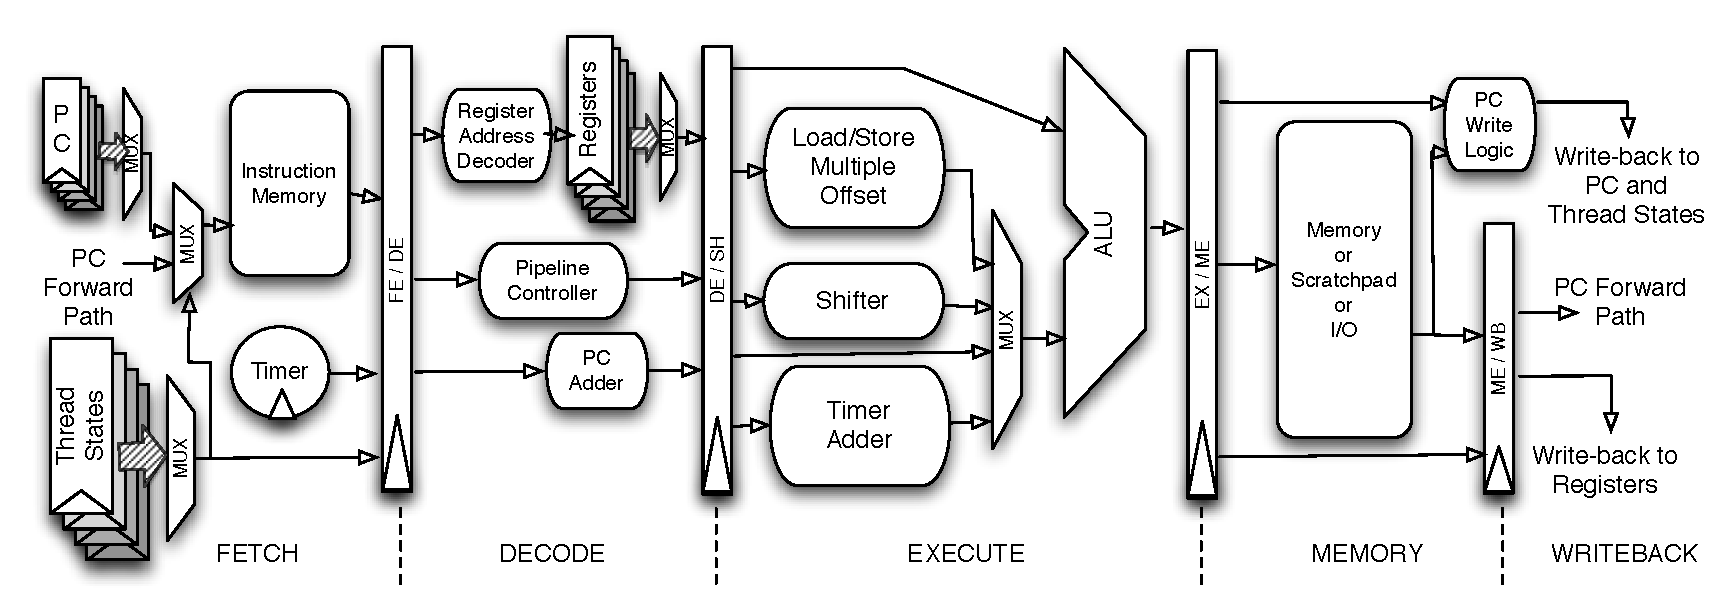
\includegraphics[scale=.54]{figs/ptarm_pipeline_five_stage}
  \end{center}
  \vspace{-20pt}
  \caption{Block Level View of the PTARM 5 stage pipeline}
  \label{fig:ptarm_pipeline_five_stage}
\end{figure}

%The \emph{fetch} and \emph{decode} stages setup the data operands and control signals for the later stages to execute the instruction.
The \emph{fetch stage} of the pipeline selects the correct PC according to which thread is executing, and passes the address to instruction memory. 
The PC forward path forwards a loaded address from main memory for instructions that load to R15, which causes a branch.
We will discuss the need for the forwarding path below when we describe the \emph{writeback stage}.
A simple $log(n)$ bit upcounter is used to keep track of which thread current to fetch.

The \emph{decode stage} contains the pipeline controller which does the full decoding of instructions and sets the correct pipeline signals to be propagated down the pipeline.
Most of ARM instructions are conditionally executed, so the pipeline controller first checks the condition bis to determine whether the instruction is to be executed or not.  
Typically the controller needs to know the current instructions in the pipeline to detect the possibility of pipeline hazards and stall the current instruction.
However,in a thread-interleaved pipeline, other instructions down the pipeline are from threads, thus the controller logic is greatly simplified. 
It simply decodes the instruction to determine the correct signals to send to the data-path and multiplexers down the pipeline. 
A small decoding logic, the \emph{register address decoder}, is inserted in parallel with the controller to decode the register addresses from the instruction bits.  
Typical RISC instruction sets, such as MIPS, set the encoding of instruction bits so the register operands have a fixed location for all instruction types.
However, in the ARM instruction set, certain instructions encode the register read address at different bit locations of the instruction.
For example, ARM data-processing register shift instructions reads a third operand from the register to determine the shift amount.
Store instructions also read a third register to obtain the register value that is stored to memory. 
However, both instructions have different bit locations in the instruction encoding to determine what register to read from.
Thus, a small register address decoding logic is inserted for a quick decoding of the register addresses from the instruction bits.
The \emph{PC Adder} is used to increment the PC.
%FIXME: Talk about the design of the ISA to optimize pipeline implementation, which in our case did not make things easier
The ARM ISA programmer's model states that reading from R15 reads the current PC+8, the PC adder not only increments the PC by 4 to get the potential next PC, but it also increments the current PC by 8 to be used as an operand. 
Single threaded pipelines need to increment the PC immediately in the fetch stage to prepare for the next instruction fetch.  
For thread-interleaved pipelines, since the next PC from the current thread is not needed until several cycles later, it doesn't need to be in the fetch stage. 
But because we need the results of PC+8 as a data operand, it is placed in the decode stage. 
The \emph{timer} is a hardware counter clocked to the processor clock which is used to implement the timing instructions mentioned in chapter~\ref{chapter:programming_models}.
The timer contains a 64 bit value that represents nanoseconds, and starts at 0 when the pipeline starts up.  
The time value is latched in the decode stage as the subsequent stages use it for timer manipulation.

The \emph{execute}, \emph{memory} and \emph{writeback} stages execute the instruction and commits the result. 
The \emph{execute} stage contains mostly execution units and muxes that select the correct operand and feeds it to the ALU.  
The ARM ISA assumes a built in shifter to shift the operands before operations, so a 32 bit \emph{shifter} is included to shift the operands before the ALU.   
The \emph{load/store multiple offset} logic block is used to calculate the offset of load/store multiple instructions.
The load/store multiple instruction uses a 16 bit vector to represent each of the 16 general purpose registers.
The bits that are set in that bit vector represents a load/store on that register.
The an offset is added to the base memory address for the instruction, and that offset depends on how many bits are set. 
Thus, the load/store multiple offset logic block does a bit count on the bit vector and adjusts the offset to be passed into the ALU for load/store multiple instructions.
The \emph{timer adder} logic block is a 32 bit add/subtract unit.
Time in the pipeline is a 64 bit value representing nanoseconds. 
Thus, any timing instruction that interacts with the timer in the pipeline needs to operate on 64 bit values.
We could have reuse the existing ALU at the expense of having all timing instructions take an additional pass through the pipeline.
But we chose to include an addition add/subtract unit specifically for the implementation of the delay\_until instruction so it can check for deadline expiration every cycle, which we will discuss in detail in section~\ref{sec:ptarm_instructions} when we show how delay\_until is implemented.    
A 32 bit \emph{ALU} does most of the logical and arithmetic operations, including data-processing operations and branch address calculations.
The results is passed to the \emph{memory stage}, which either uses it as an address to interact with the data memory, or forwards it along to the \emph{writeback stage} to commit back to the registers.

\begin{wrapfigure}{r}{0.5\textwidth}
  \vspace{-20pt}
  \begin{center}
    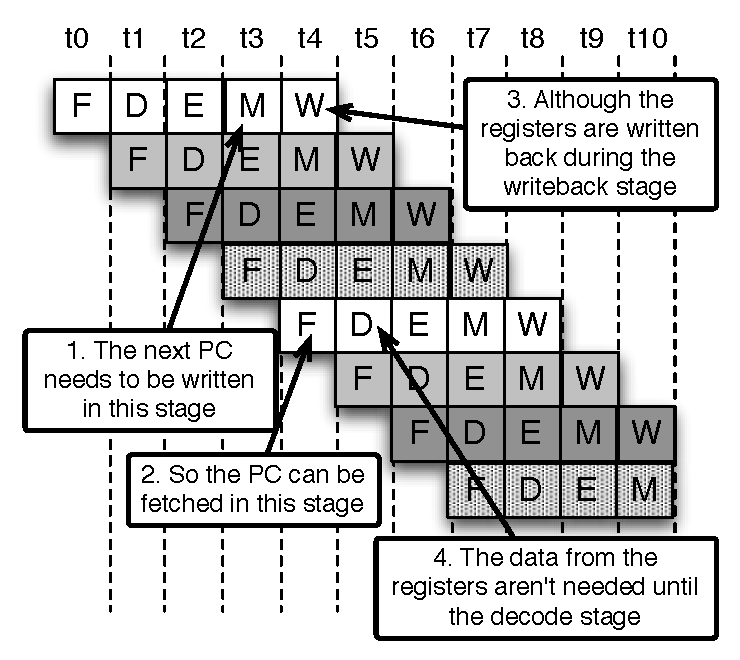
\includegraphics[scale=.65]{figs/four_thread_pipeline}
  \end{center}
  \vspace{-20pt}
  \caption{Four thread execution in PTARM}
  \label{fig:four_thread_pipeline}
  \vspace{-10pt}
\end{wrapfigure}      
%Although the register values are committed in the write back stage, the next PC address needs to be written back earlier. 
Figure~\ref{fig:four_thread_pipeline} shows an execution sequence of the four thread five stage pipeline.
The instruction in the fetch stage belongs to the same thread as the instruction in the writeback stage.
This does not cause any data hazards because the data from the registers will not be read until the decode stage. 
But committing the PC at the writeback stage would result in a control hazard because the PC would not be ready for the subsequent fetch.
For most instructions, the next PC calculation is completed before the memory stage, so we move the PC commit one stage earlier so the next instruction can be fetched.
However, the ARM ISA allows instructions to write to register 15 (PC), which acts as a branch to the value written to R15.   
This means a load instruction can write to R15 and cause a branch whose target is not known until after the memory read.   
Thus, a PC forwarding path is added to forward the PC back from memory if a load instruction writes to R15.  
The forwarding path does not cause any timing analysis difficulties because the statically the forwarding path is only used when a load instruction writes to R15, which can be statically determined. 
Also, this causes no stall in the pipeline, and does not effect the timing of any following instructions. 
This allows us to interleave four threads in our five stage pipeline instead of five.    

\section{Memory Hierarchy} 
The instruction memory is currently composed of an instruction scratchpad and a boot ROM. 
The boot ROM \todo{mention bootROM size} is shared between all the threads and contains the initialization code for each thread. 
It also contains the exception vector table that stores entries for handling different exceptions that occur in the pipeline, along with some of the exception handlers. 
The instruction scratchpad \todo{size?} is currently logically divided into five regions. 
Each of the threads contains its own private instruction region, and a shared region where all threads can access.
Both the boot ROM and instruction scratchpad are also synthesized to FPGA block RAMs, and both give single cycle access latencies.

The data memory 

\section{Instruction Implementations}
\label{sec:ptarm_instructions}
In this section we go into more details on how each instruction type is implemented and how each hardware block in the pipeline shown in figure~\ref{fig:ptarm_pipeline_five_stage}. 
We will go through different instruction types and discuss the timing implications each instruction in our implementation.
%FIXME: Talk about the difference between thread cycle and regular processor cycle
We will summarize with a table with all instructions and the cycle count it takes to execute them.
   
\subsection{Data-Processing}
We begin by explaining how data-processing instructions are implemented.
These instructions are used to manipulate register values by executing register to register operations. 
Most data-processing instructions take two operands.
One operand is always a register value, the second operand is labeled the shifter operand. 
The shifter operand could be an immediate value or a register value, both which can be shifted to form the final operand that is fed into the ALU.
Figure~\ref{fig:data_processing_pipeline_implementation} explains how data-processing instructions are executed through the pipeline.
\begin{figure}
  \vspace{-20pt}
  \begin{center}
    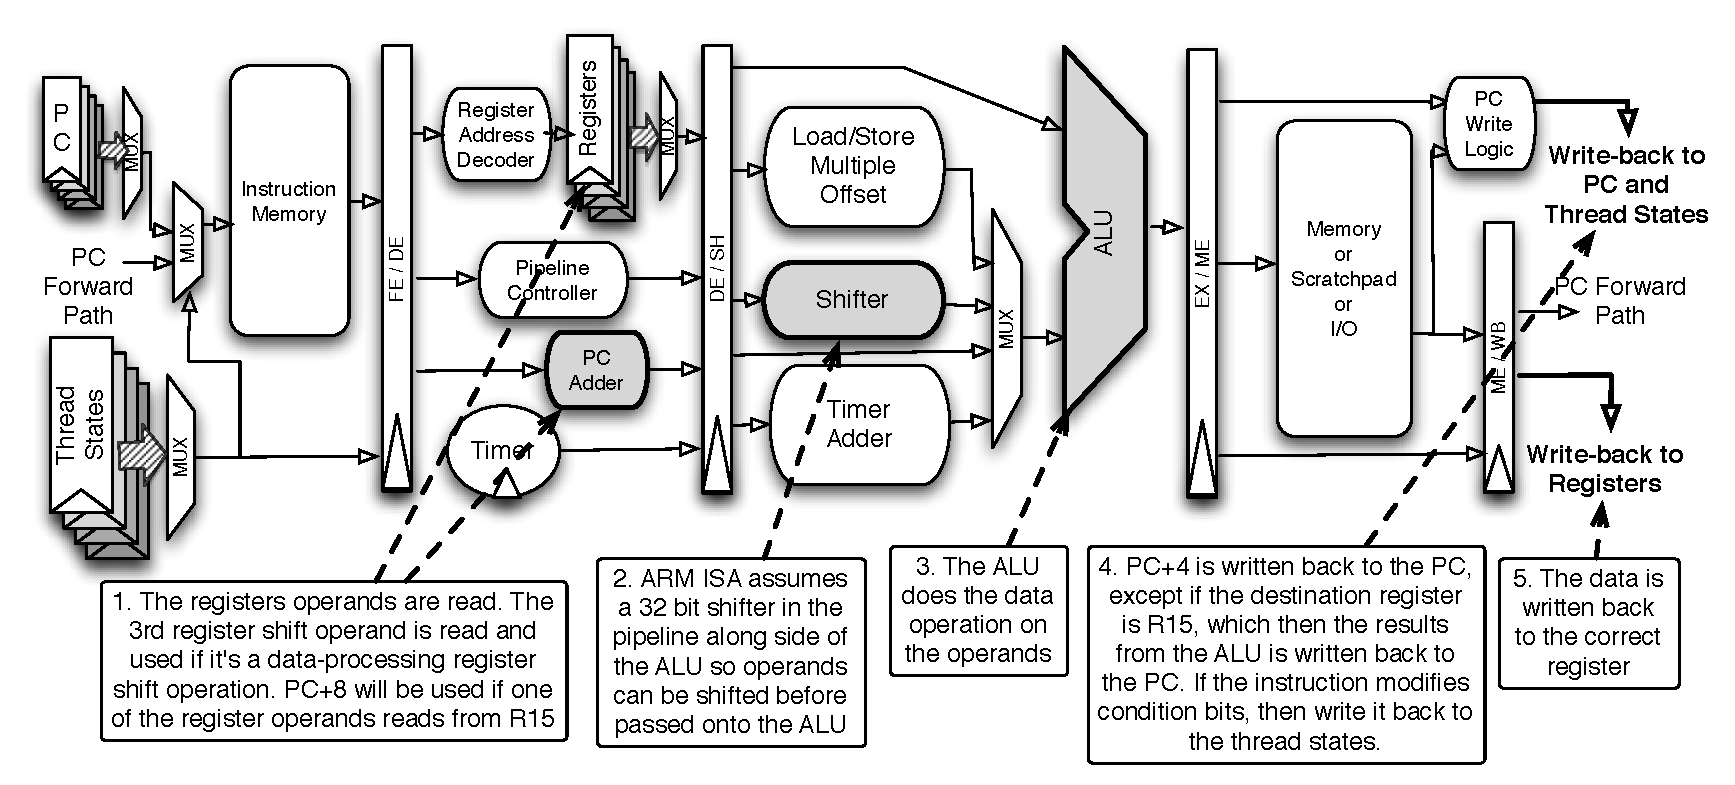
\includegraphics[scale=.54]{figs/data_processing_pipeline_implementation}
  \end{center}
  \vspace{-20pt}
  \caption{Data Processing Instruction Execution in the PTARM Pipeline}
  \label{fig:data_processing_pipeline_implementation}
\end{figure}

Because R15 is PC, so data-processing instructions that use R15 as an operand will read the value of PC+8 as the operand. 
Any instruction that uses R15 as the destination register will trigger a branch to the result of the computation.
As discussed earlier, our pipeline commits the next PC in the memory stage, so to trigger a branch from data-processing instructions simply means storing back the results from the ALU as the next PC.
In our thread-interleaved pipeline, when the next PC from the current thread is fetched, it will contain already contain the target address to branch to when we issue a data-processing instruction that writes to R15. 

Data processing instructions can also update the program condition code flags that are stored in the thread state. 
The condition code flags are used to predicate execution for ARM instructions, and consists of four bits: Zero (Z), Carry (C), Negative (N) and Overflow (V). 
The high four bits of each instruction forms a conditional field that is checked against the thread state condition code flags to determine whether or not the instruction is executed. 
The conditional execution for each instruction is checked in the pipeline controller. 
Data-processing instructions provide a mechanism to update the condition code flags according to the results of data operations.
The instructions that update the flags do not write any data back to the registers, they simply update the condition code flags.

All data-processing instructions only take one pass through the pipeline, even instructions that read from or write to R15, so all data-processing instructions take one thread cycle to execute. 
\subsection{Branch}
\begin{figure}
  \vspace{-20pt}
  \begin{center}
    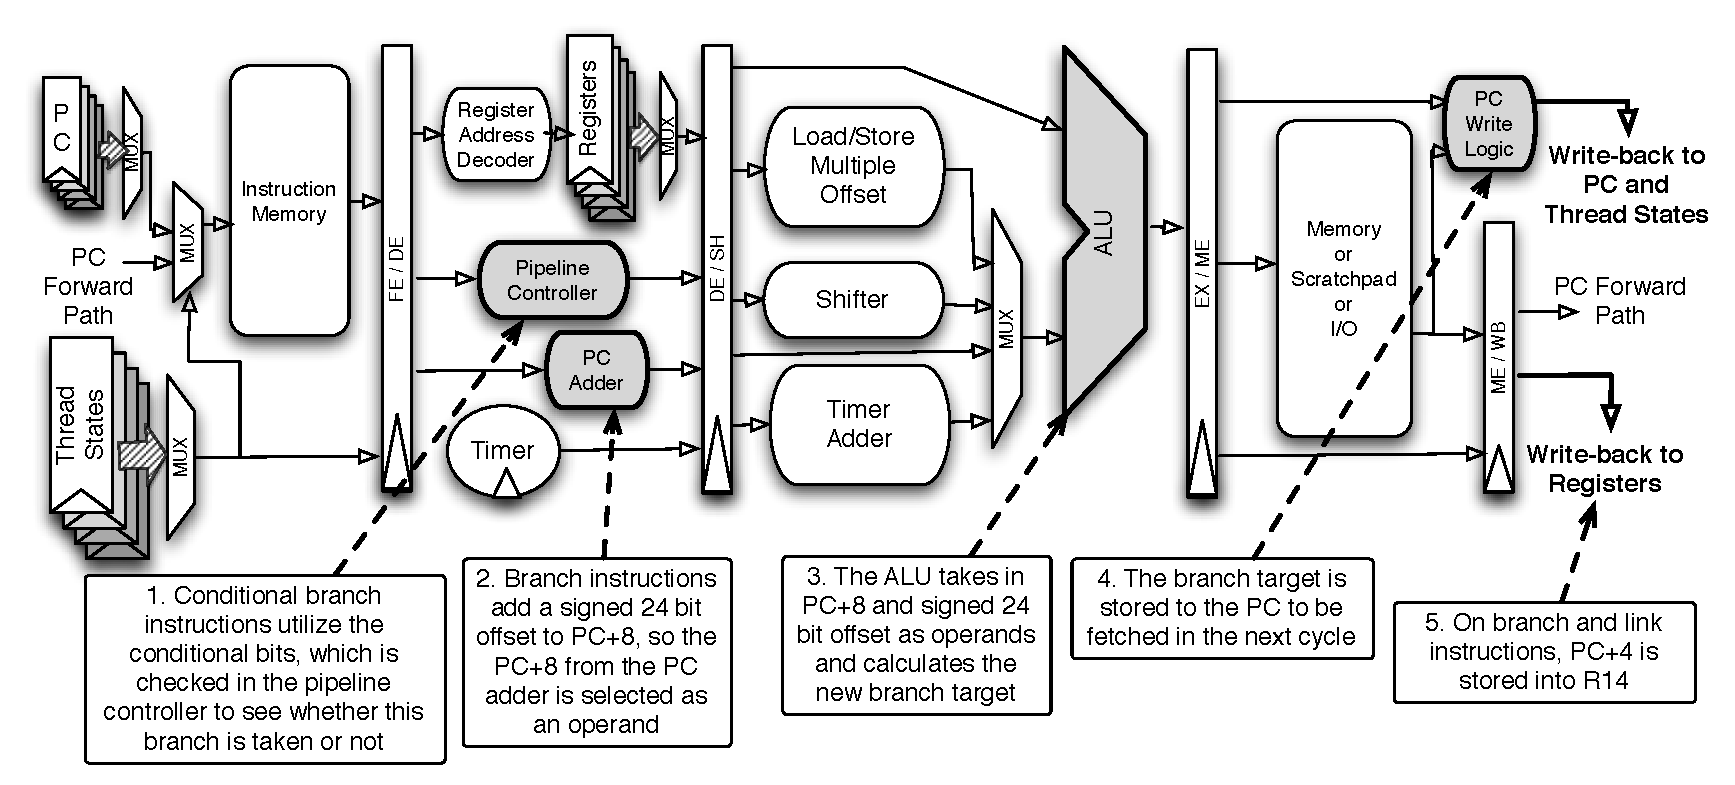
\includegraphics[scale=.54]{figs/branch_pipeline_implementation}
  \end{center}
  \vspace{-20pt}
  \caption{Branch Instruction Execution in the PTARM Pipeline}
  \label{fig:branch_pipeline_implementation}
\end{figure}
Branch instructions in the ARM can conditionally branch forward or backwards by up to 32MB.
There is no explicit conditional branch instruction in ARM.
Conditional branches are implemented using the ARM predicated instruction mechanism.
So the condition used to determine if a conditional branch is taken is simply the condition code flags in the thread state. 
Figure~\ref{fig:branch_pipeline_implementation} show how branch instructions are executed in the thread-interleaved pipeline.

The branch instructions for the ARM ISA calculate the branch target address by adding a 24 bit signed offset, specified in the instruction, to the current PC incremented by 8. 
Thus, the PC adder, in addition to incrementing the PC by the conventional offset of 4, also increments the PC by 8, to be used as an operand for the ALU to calculate the target branch address.
Once the address is calculated, it is written back to its thread's next PC ready to be fetched. 
If the instruction is a branch and link ($bl$) instruction, PC+4 is propagated down the pipeline and written back to the link register (R14).   

All branch instructions, whether conditionally taken or not, all take only one thread cycle to execute.
But more importantly, the next instruction after the branch, whether it is a conditional branch or not, is not stalled or speculatively executed. 
The execution time of instructions from the same thread after the branch is not stalled nor affected by the branch instruction.  
The thread-interleaved pipeline simplified the implementation of the branch instruction and control hazard handling logic, as the pipeline will not need the results of the branch target address calculation the very next processor cycle.  
Instead, instructions from other threads will be fetched before the results of the branch is needed.

\subsection{Memory Operations}

\subsubsection{Load/Store Registers}
\begin{figure}
  \vspace{-20pt}
  \begin{center}
    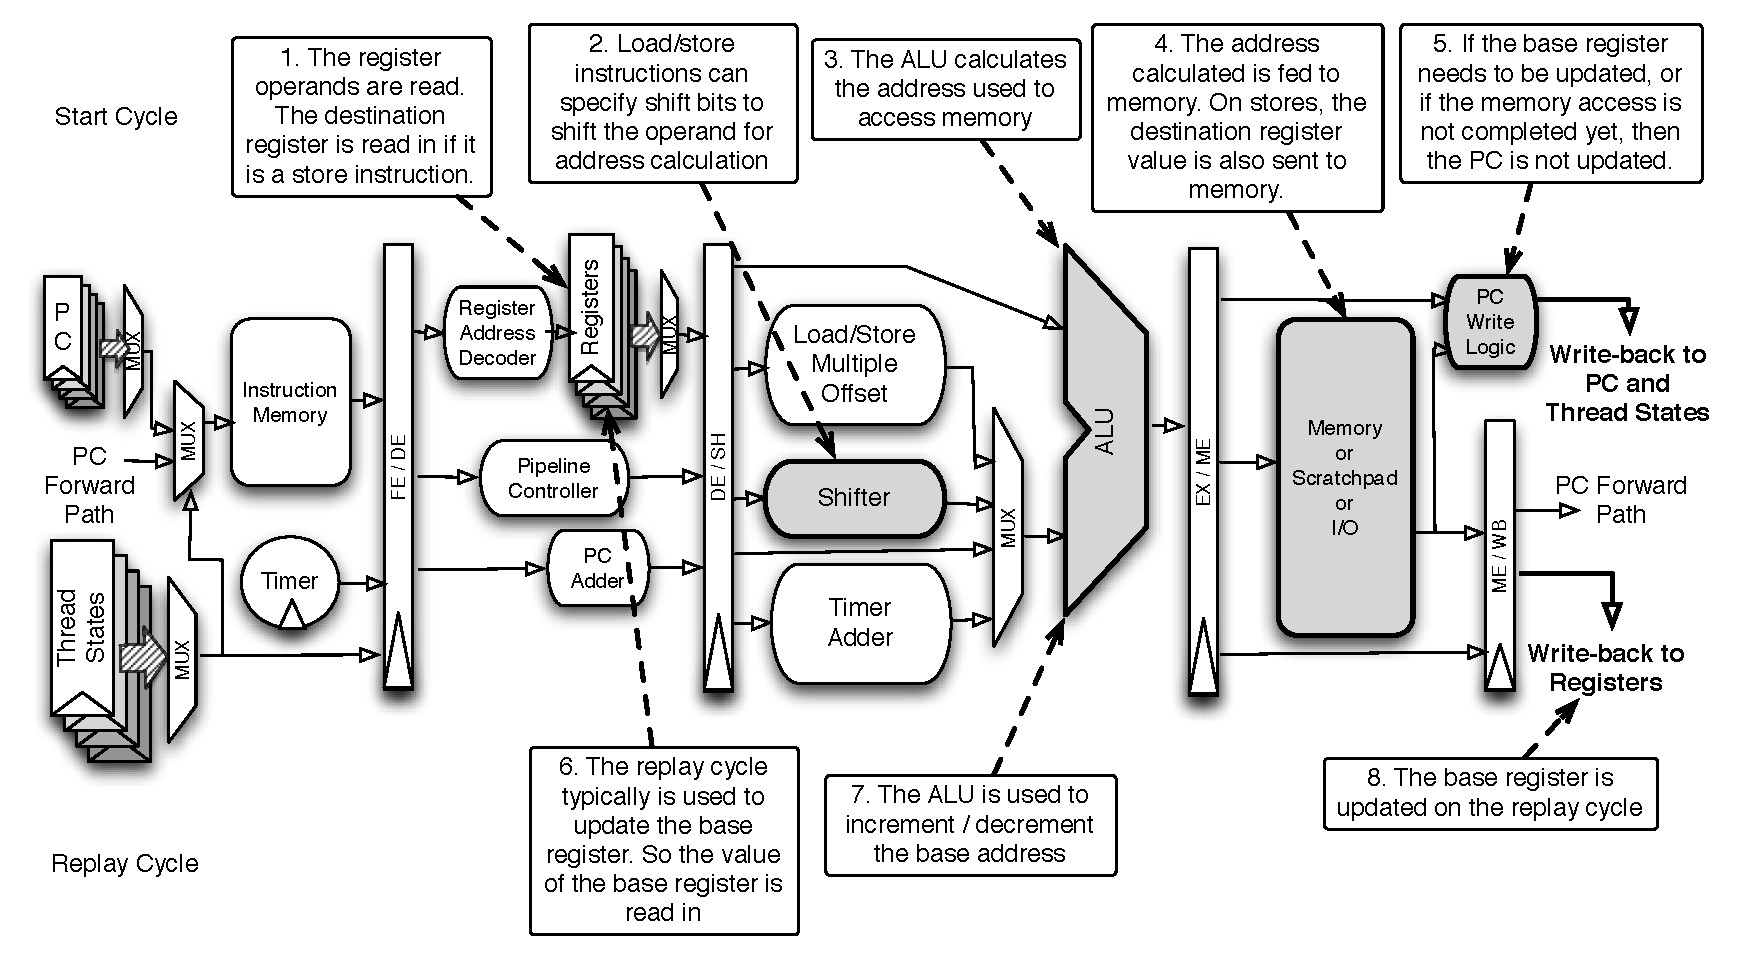
\includegraphics[scale=.54]{figs/ldstr_pipeline_implementation}
  \end{center}
  \vspace{-20pt}
  \caption{Load/Store Instruction Execution in the Ptarm Pipeline}
  \label{fig:ldstr_pipeline_implementation}
\end{figure}
Very similar to data processing instructions, except the ALU results gets used for the memory access.
Write about incrementing the base register 

For load and store instructions, the memory access address is formed by combining a base register and an offset value. 
ARM also specifies the ability to update the base register after any memory operation. 
This compacts code that reads arrays, as a load or store instruction can access memory and updates the base register so the next memory access is done on the updated base register.
ARM calls these pre-indexed and post-indexed addressing modes. 
Pre-indexed addressing mode calculates the memory address by first using the value of the base register and offset, then updating the base register. 
Post-indexed addressing mode first updates the base register, then uses the updated base register value along with the offset to form the memory address. 
The base register could be incremented or decremented when it is being updated.   
Because there is only one write port to our register file however, we cannot simultaneously write back a load result from memory and the updated base register to the register file in a single cycle. 
As a result,

\subsubsection{Load/Store Multiple}

\begin{figure}
  \vspace{-20pt}
  \begin{center}
    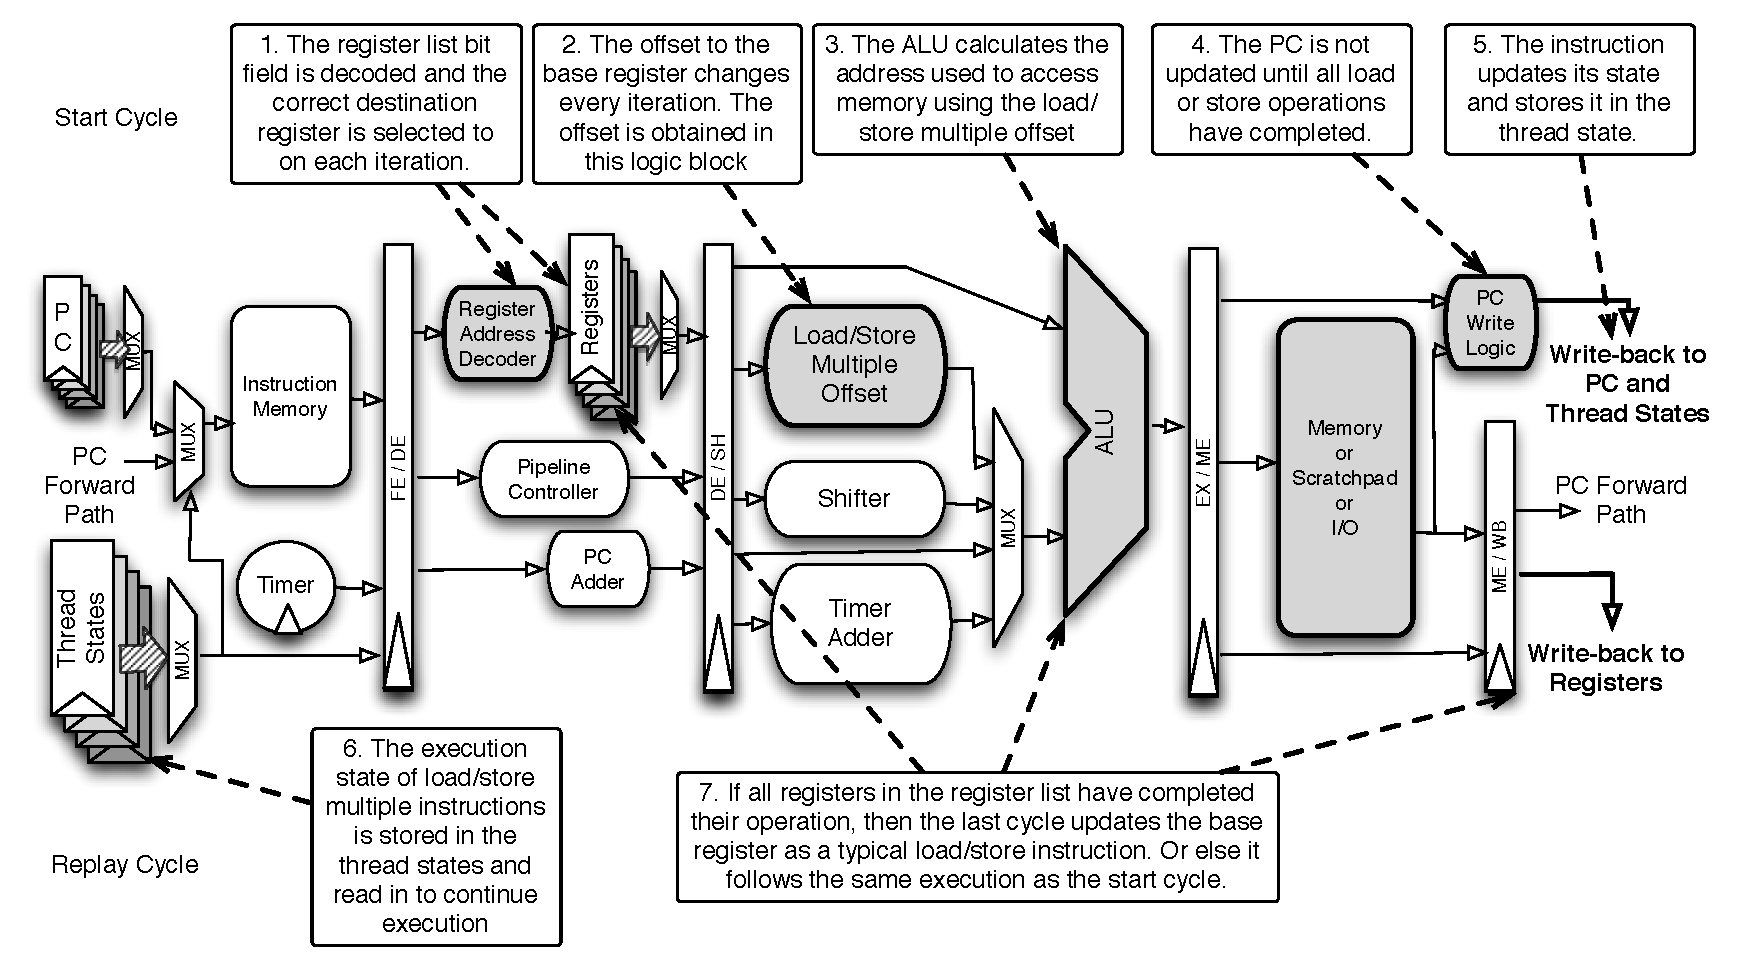
\includegraphics[scale=.54]{figs/ldstrm_pipeline_implementation}
  \end{center}
  \vspace{-20pt}
  \caption{Load/Store Multiple Instruction Execution in the PTARM Pipeline}
  \label{fig:ldstrm_pipeline_implementation}
\end{figure}

\subsubsection{Load to PC}    
  
\begin{figure}
  \vspace{-20pt}
  \begin{center}
    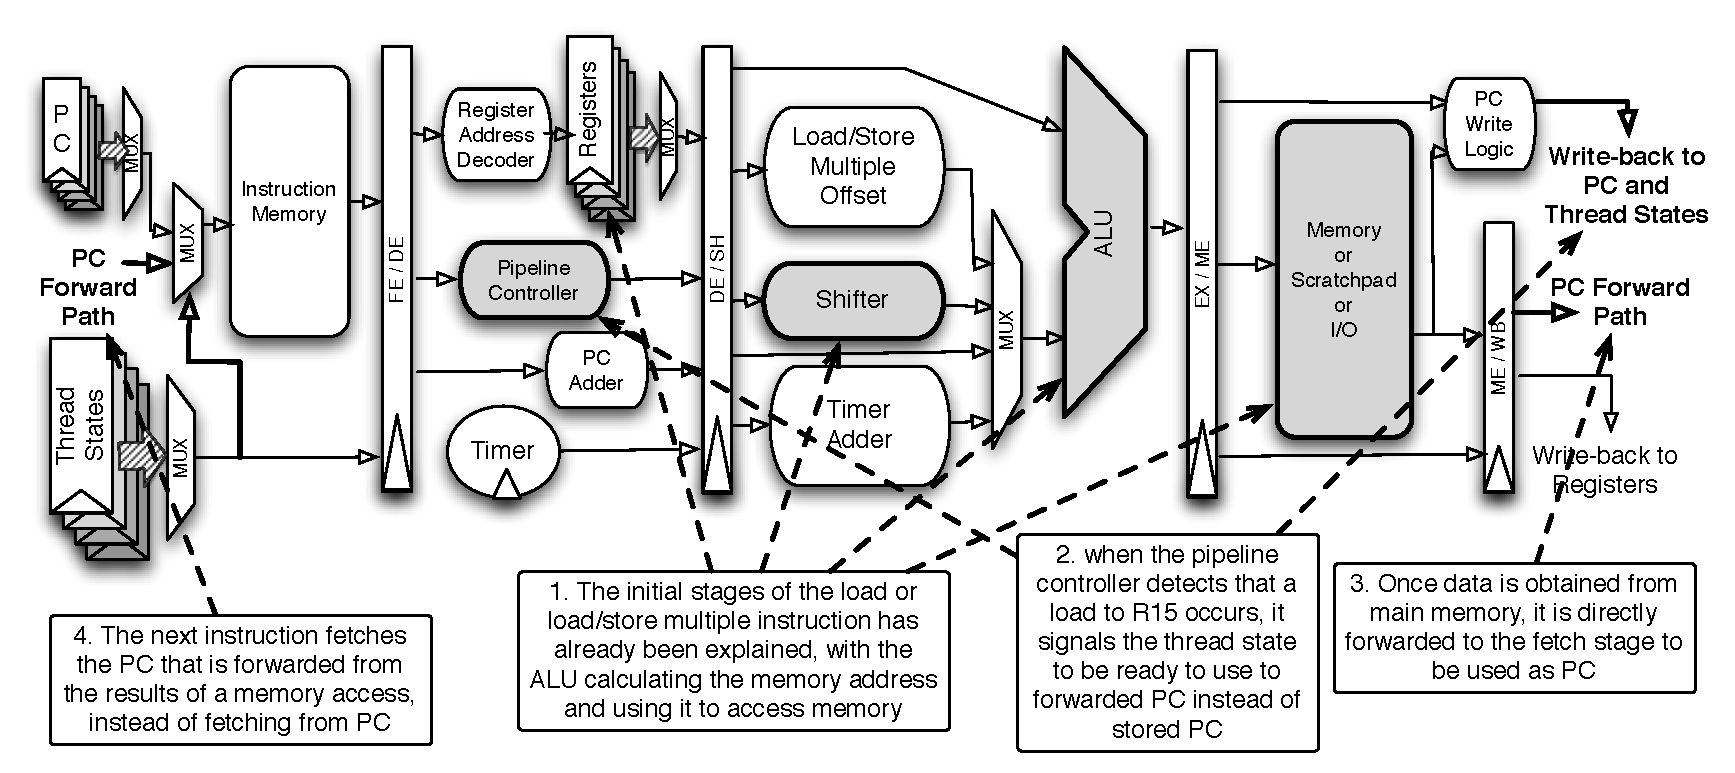
\includegraphics[scale=.54]{figs/ld_to_pc_pipeline_implementation}
  \end{center}
  \vspace{-20pt}
  \caption{Load to R15 Instruction Execution in the PTARM Pipeline}
  \label{fig:ld_to_pc_pipeline_implementation}
\end{figure}
\subsection{Exception Handling}

\subsection{Timing Instructions}

\subsubsection{Get\_Time}    

\begin{figure}
  \vspace{-20pt}
  \begin{center}
    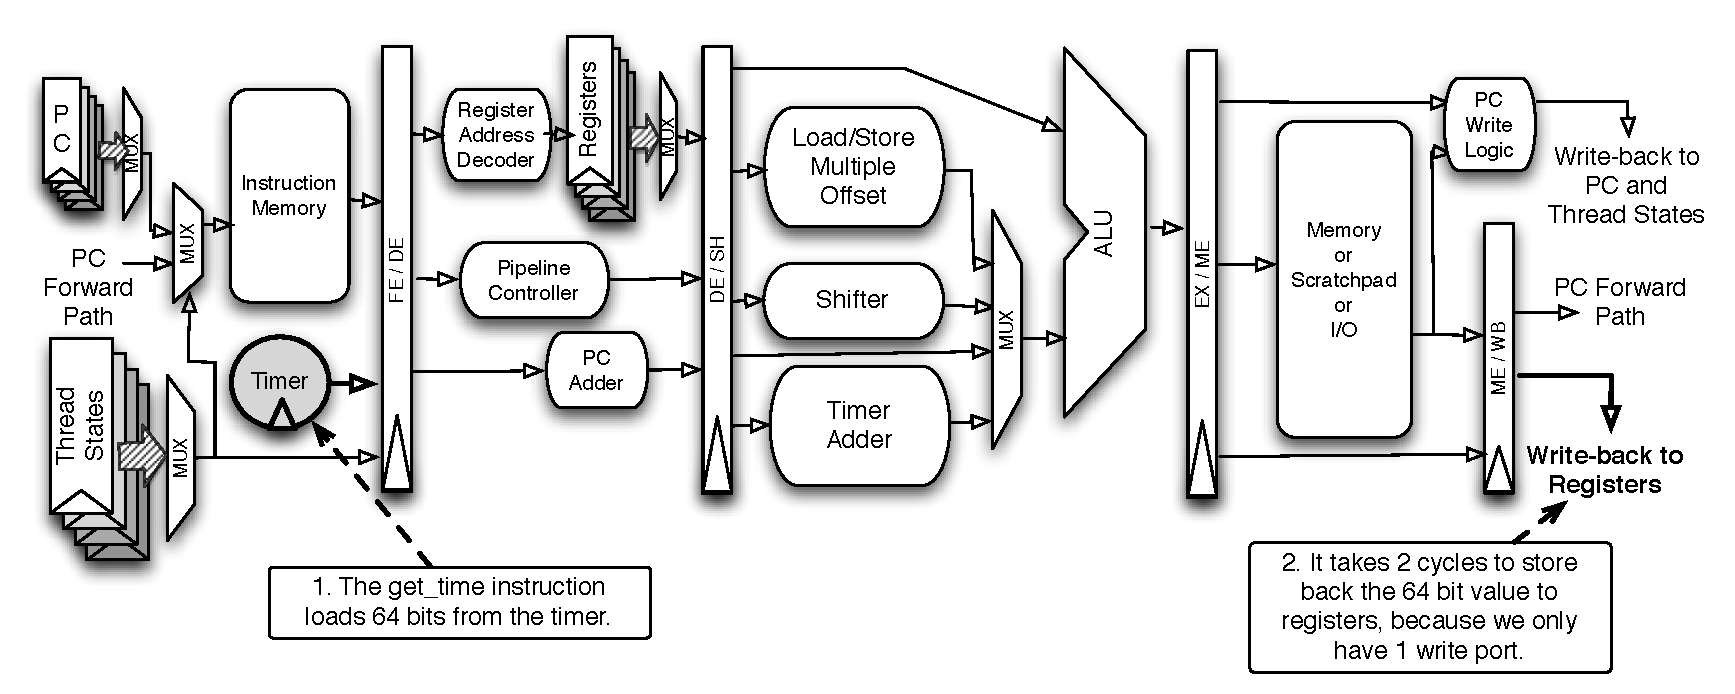
\includegraphics[scale=.54]{figs/get_time_pipeline_implementation}
  \end{center}
  \vspace{-20pt}
  \caption{Get\_Time Instruction Execution in the PTARM Pipeline}
  \label{fig:get_time_pipeline_implementation}
\end{figure}

\subsubsection{Delay\_Until}    

\begin{figure}
  \vspace{-20pt}
  \begin{center}
    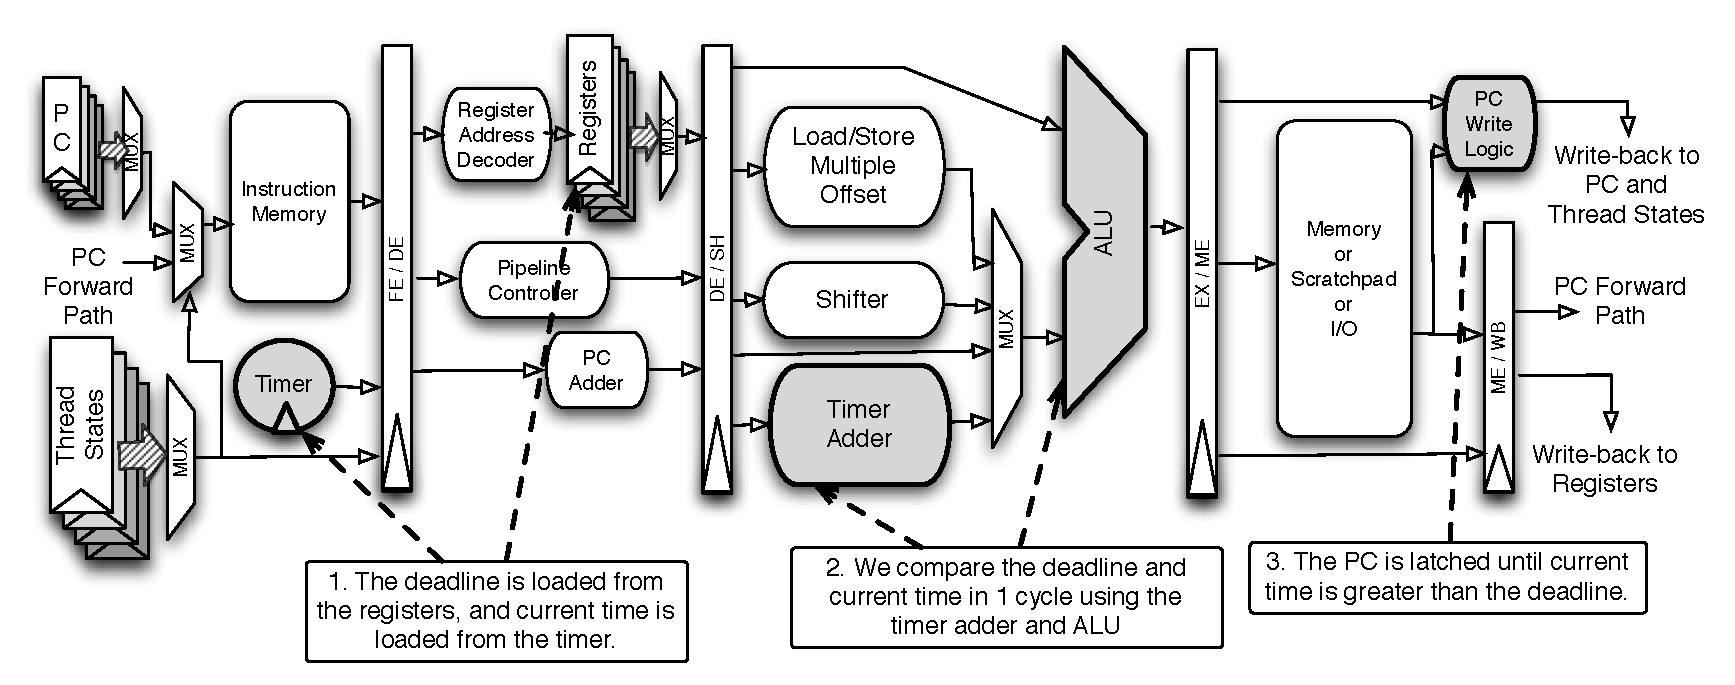
\includegraphics[scale=.54]{figs/delay_until_pipeline_implementation}
  \end{center}
  \vspace{-20pt}
  \caption{Delay\_Until Instruction Execution in the PTARM Pipeline}
  \label{fig:delay_until_pipeline_implementation}
\end{figure}

\subsubsection{Exception\_on\_Expire, Deactivate\_Exception}    

\section{Worst Case Execution Time Analysis}
\label{sec:wcet}
 
\section{PTARM VHDL Soft Core}
Our pipeline can be clocked up to $100MHz$ when synthesized to a Virtex-5 lx110t FPGA.

Talk about I/O devices, including UART, DVI controller and Interface with DDR2 DRAM controller  

\section{PTARM Simulator}
\label{sec:ptarm_sim}

Talk about experimentation with DMA and memory hierarchy





